\section{Results}


\subsection{Classifying behaviors}

Here we used a Random Tree Classifier based on wavelet angles in order to classify behaviors. We used 25 wavelet features from joint angles with frequencies between 1 to \SI{50}{Hertz}. It results in an accuracy of around 99.1\% on a test set. We looked at the most important features and find out that the angle LF leg Coxa roll was the most predictive joint angles, followed by the angle LF leg Coxa and the angle LF leg Femur. We see that the most important features are at the basis of the fly's leg, discriminating probably walking from resting behaviors, as those 2 are the most frequent behaviors. 

\subsection{Identifying correlations of individual neurons}

After having standardized the neuronal data, we first computed the mean activity in all neurons during the different behaviors too see whether some activity were triggering higher activity in all neurons. But as we can see in Figure~\ref{fig:mean_neuron_behav_matrix} we do not have higher overall neuron activity for specific behavior. 

\begin{figure}[htbp]
	\begin{center}
		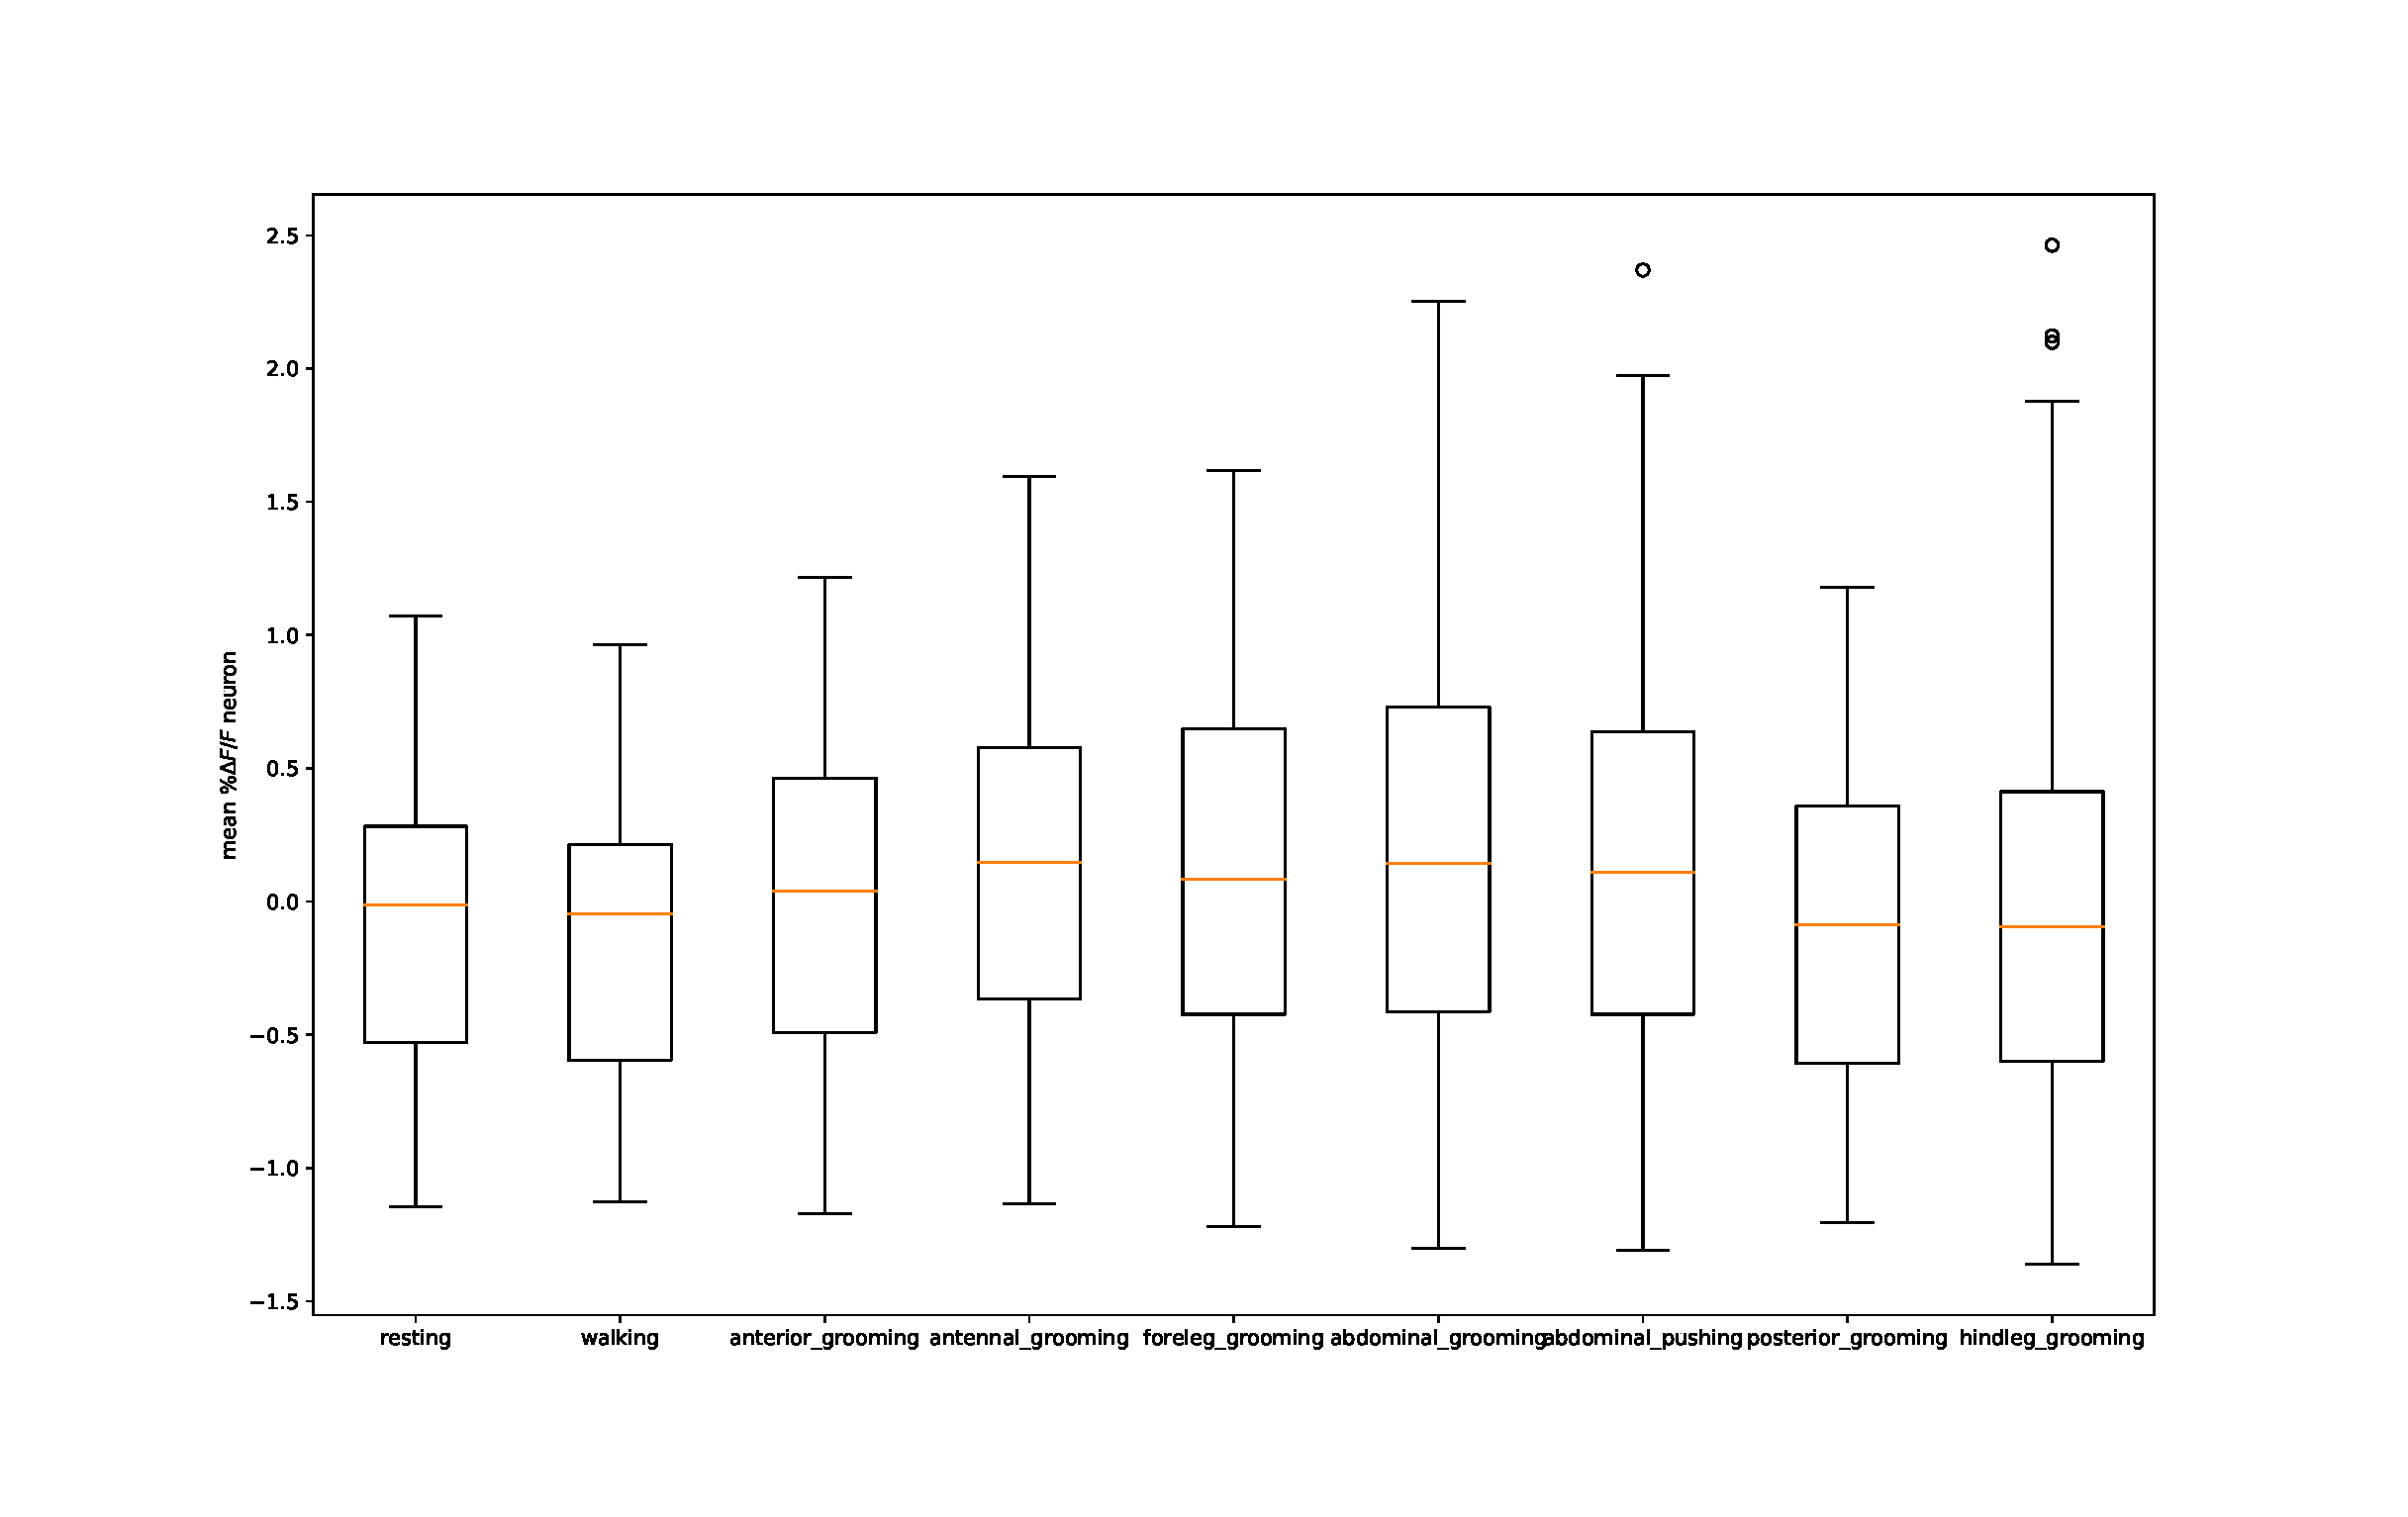
\includegraphics[width=\textwidth]{mean_neuron_behav_matrix}
	\end{center}
	\caption{Boxplot of mean activity for all neurons of different behaviors.}
	\label{fig:mean_neuron_behav_matrix}
\end{figure}

Thus, in order to have a visual representation of specific neuronal activity, we plot a matrix with all neurons and their activity levels in Figure~\ref{fig:neuron_behav_matrix} 

\begin{figure}[htbp]
	\begin{center}
		\includesvg[width=\textwidth]{neuron_behav_matrix}
	\end{center}
	\caption{Matrix with each neuron and its relative activity with different behaviors.}
	\label{fig:neuron_behav_matrix}
\end{figure}

The matrix does not give us lots of insights about a possible higher neuronal activity for a specific behavior. Although we can see some higher activation (more yellowish) neurons for certain behaviors we cannot conclude anything for that so we will use statistics to discover significant neurons coding for specific behavior. 

Thus we have run an ANOVA and Tukey test for significant differences and we found that the neurons in Table~\ref{table:statistical_table} have a significant difference in mean activity when doing the specific behavior cited in the table compared to all other behaviors. 

\begin{table}[htbp]
	\sffamily
	\arrayrulecolor{white}
	\arrayrulewidth=1pt
	\renewcommand{\arraystretch}{1.5}
	\rowcolors[\hline]{1}{.!50!White}{}
	\centering
	\begin{tabular}{@{} B|A @{}}
		\cellcolor{ForestGreen}\arraycolor{White}\bfseries Neuron &
		\cellcolor{ForestGreen}\arraycolor{White}\bfseries Behavior \\   
		\arraycolor{Black}
		2 & resting \\
		3 & resting \\
		62 & resting \\
		80 & resting \\
		81 & resting \\
		25 & foreleg grooming \\
		36 & foreleg grooming \\
		42 & abdominal pushing \\
		71 & abdominal pushing \\
		86 & abdominal pushing \\
		109 & abdominal pushing \\
		122 & abdominal pushing \\
		113 & antennal pushing \\
		122 & abdominal grooming \\
	\end{tabular}
	\label{table:statistical_table}
	\caption{Statistical significant mean difference between mean neuronal activity and behavior.}
\end{table}

Having those results we group neurons by their significant behavior and plot them against time. For example in Figure~\ref{fig:trial_7_resting} we plotted neurons that have significantly different means in the resting state against time. We added in light orange when the fly is resting and we choose trial 7 for example but it worked for all trials equally. We also plotted in Figure~\ref{fig:trial_7_antennal_grooming} the antennal grooming activity linked to neuron 113. 

\begin{figure}[htbp]
	\begin{center}
		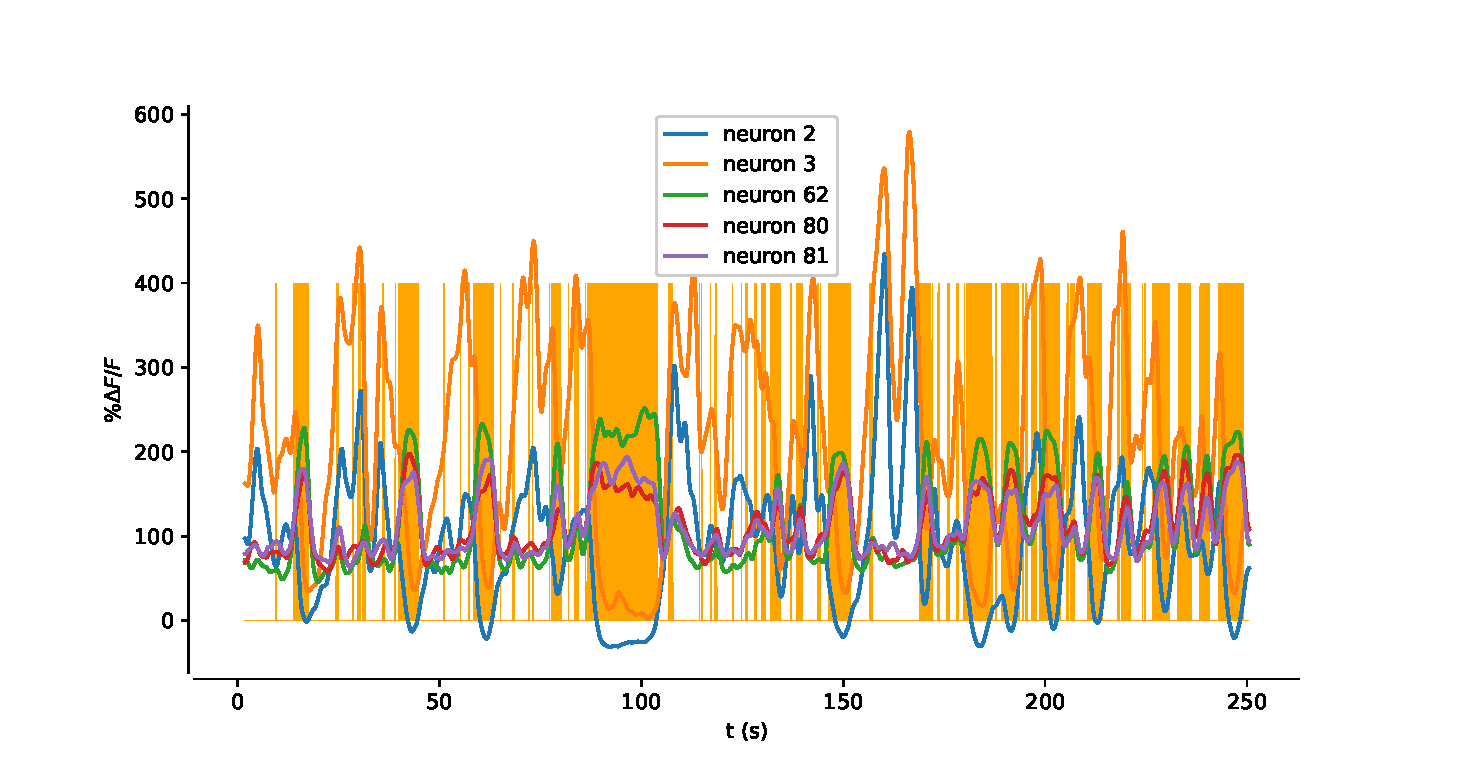
\includegraphics[width=\textwidth]{trial_7_resting}
	\end{center}
	\caption{Neurons activity for trial 7 with the resting state in orange.}
	\label{fig:trial_7_resting}
\end{figure}

\begin{figure}[htbp]
	\begin{center}
		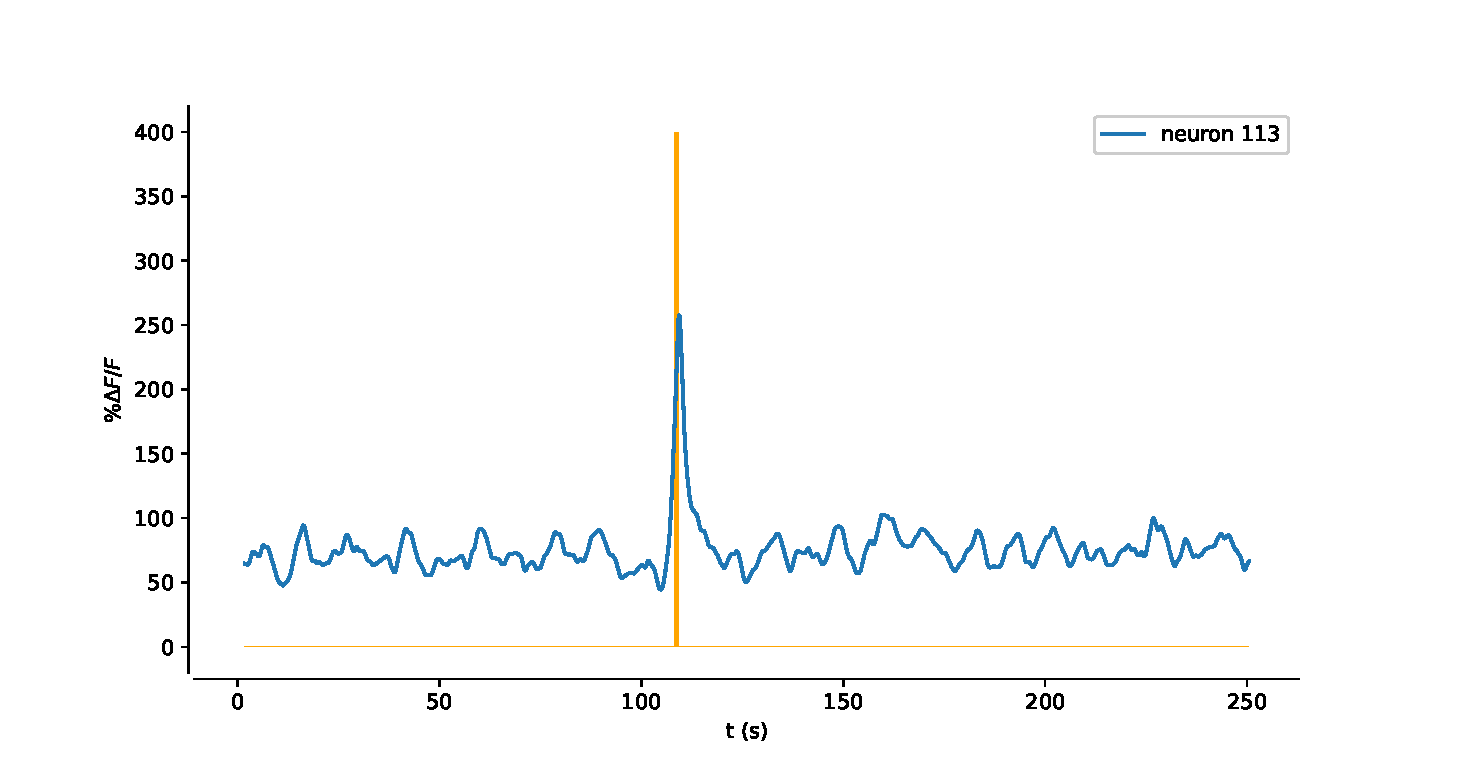
\includegraphics[width=\textwidth]{trial_7_antennal_grooming}
	\end{center}
	\caption{Neuron 113 activity for trial 7 with the antennal grooming state in orange.}
\label{fig:trial_7_antennal_grooming}
\end{figure}

We have to be careful when analyzing those data because we have seen in the methods that some behaviors have only very few data. Here for example we analyzed the walking behavior and found out that for 58 out of the 123 neurons it was significantly different in means from all other neurons except hind leg grooming. Hind leg grooming is a really rare behavior only happening 2 times in our reduced behavioral dataset and thus if we remove it from our analysis there would be those 58 neurons having a significant difference in means with all other behaviors. We will restrain our analysis of statistics here as we will see later by classifying behaviors which are the important neurons coding for the walking behavior. 

In Table~\ref{tab:spearman_table} we retain Spearman correlation that are higher than the absolute value of 0.5 to observe moderately correlated joint angles to neurons. We only kept values where the p-value of that correlation was lower than 5\%. 

\begin{table}[htbp]
	\sffamily
	\arrayrulecolor{white}
	\arrayrulewidth=1pt
	\renewcommand{\arraystretch}{1.5}
	\rowcolors[\hline]{1}{.!50!White}{}
	\centering
	\begin{tabular}{@{} B|A|A @{}}
		\cellcolor{ForestGreen}\arraycolor{White}\bfseries Neuron &
		\cellcolor{ForestGreen}\arraycolor{White}\bfseries Angle &
		\cellcolor{ForestGreen}\arraycolor{White}\bfseries Correlation \\   
		\arraycolor{Black}
		36 & LM leg Femur & 0.63 \\
		25 & LM leg Femur & 0.61 \\
		101 & RH leg Coxa roll & 0.58 \\
		117 & LM leg Femur & 0.57 \\
		65 & LM leg Femur & 0.55 \\
		102 & LM leg Femur & 0.55 \\
		63 & LM leg Femur & 0.55 \\
		25 & LF leg Femur & 0.50 \\
		36 & RM leg Femur & 0.50 \\
		36 & LF leg Femur & 0.50 \\
		36 & LM leg Tarsus & -0.57 \\
		25 & LM leg Tarsus & -0.57 \\
		25 & RH leg Coxa roll & -0.55 \\
		102 & RH leg Coxa roll & -0.52 \\
		20 & RH leg Coxa roll & -0.52 \\
		117 & LM leg Tarsus & -0.51 \\
		36 & RM leg Tarsus & -0.50 \\
	\end{tabular}
	\caption{Statistical significant mean difference between mean neuronal activity and behavior.}
	\label{tab:spearman_table}
\end{table}

We plotted in Fig~\ref{fig:spearman_neuron_36} the biggest Spearman correlation which is for neuron 36 and the left medial Femur angle.  Spearman positive correlation of 0.6347078515333816, p<0.05

\begin{figure}
	\begin{center}
		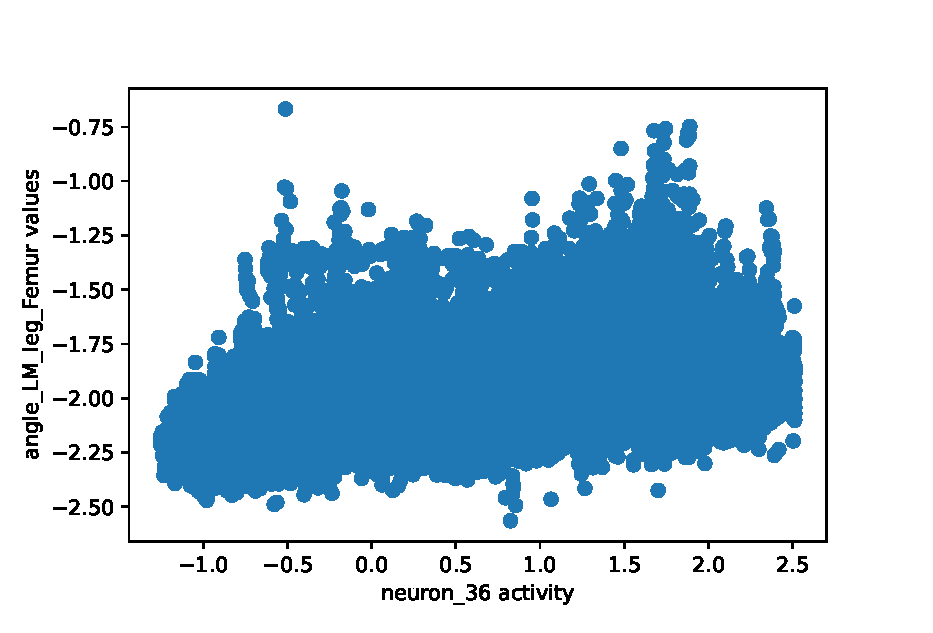
\includegraphics{spearman_neuron_36}
	\end{center}
	\caption{Spearman positive correlation of 0.6347078515333816, p<0.05 for neuron 36 for the left medial Femur.}
	\label{fig:spearman_neuron_36}
\end{figure}

As this correlation is quite small we can say that Ascending and Descending Neurons are more correlated to behavioral categories than only joint angles. From a biological perspective it can be due to the fact that those neurons encode entire behavior and joint angles result in a process involving many different neuron contributions. 

\subsection{Predicting behaviour form neuronal activity}

This part of the report present the result of the classification using logistic regression to classified walking behavior form the neuronal activity and a logistic regression and random forest classifier to classified all the behavior 
\subsubsection{One behavior : walking with logistic regression}
The first logistic regression is done one each neuron neuronal activity separately as and input and an binary variable which indicates if the fly walk or not as an output. The Table~\ref{tab::lr_single_neuron} resume the result of the regression with the 10 neurons who have the maximum accuracy.

\begin{table}[htbp]
	\sffamily
	\arrayrulecolor{white}
	\arrayrulewidth=1pt
	\renewcommand{\arraystretch}{1.5}
	\rowcolors[\hline]{1}{.!50!White}{}
	\centering
	\begin{tabular}{@{} B|B @{}}
		\cellcolor{ForestGreen}\arraycolor{White}\bfseries Neuron &
		\cellcolor{ForestGreen}\arraycolor{White}\bfseries Accuracy \\   
		\arraycolor{Black}
		32 		& 0.788		\\
		38		& 0.787		\\
		99		& 0.785		\\
		28 		& 0.784 	\\
		12 		& 0.779 	\\
		51		& 0.774		\\
		93		& 0.773		\\
		62		& 0.772		\\
		48		& 0.771 	\\
		5		& 0.768
	\end{tabular}
	\caption{Logistic regression accuracy for the 10 more accurate neuron for the differentiation of walking.}
	\label{tab::lr_single_neuron}
\end{table}

The next two Figure~\ref{fig::ow_neuron_32} and~\ref{fig::ow_neuron_38} which represent the two first neuron found in the Table~\ref{tab::lr_single_neuron}.


\subsubsection{Multiple behavior}
The logistic regression is now applied to all the neural activity to classified all the neuron. The accuracy found for this regression is $0.806$. The Table~\ref{tab::lr_multiple_neuron} shows the 10 more important neuron for each behavior.

\begin{table}[htbp]
	\sffamily
	\arrayrulecolor{white}
	\arrayrulewidth=1pt
	\renewcommand{\arraystretch}{1.5}
	\rowcolors[\hline]{1}{.!50!White}{}
	\centering
	\begin{tabular}{@{} A|C|C|C|C|C|C|C|C|C|C @{}}
		\cellcolor{ForestGreen}\arraycolor{White}\bfseries Neuron &
		\cellcolor{ForestGreen}\arraycolor{White}\bfseries 1 &
		\cellcolor{ForestGreen}\arraycolor{White}\bfseries 2 &
		\cellcolor{ForestGreen}\arraycolor{White}\bfseries 3 &
		\cellcolor{ForestGreen}\arraycolor{White}\bfseries 4 &
		\cellcolor{ForestGreen}\arraycolor{White}\bfseries 5 &
		\cellcolor{ForestGreen}\arraycolor{White}\bfseries 6 &
		\cellcolor{ForestGreen}\arraycolor{White}\bfseries 7 &
		\cellcolor{ForestGreen}\arraycolor{White}\bfseries 8 &
		\cellcolor{ForestGreen}\arraycolor{White}\bfseries 9 &
		\cellcolor{ForestGreen}\arraycolor{White}\bfseries 10 \\   
		\arraycolor{Black}
		Neuron 					& 1 & 2 & 3 & 4 & 5 & 6	& 7 & 8 & 9 & 10 \\
		Resting 				& 0 & 62 & 109 & 48 & 100 & 101	& 73 & 30 & 41 & 36 \\
		Walking					& 28 & 109 & 100 & 103 & 117 & 48 & 101 & 23 & 39 & 38 \\
		Abdominal pushing		& 22 & 7 & 8 & 20 & 40 & 116 & 105 & 30 & 23 & 42 \\
		Anterior grooming 		& 34 & 89 & 99 & 84 & 44 & 38 & 100 & 51 & 65 & 119 \\
		Posterior grooming 		& 118 & 120 & 47 & 33 & 43 & 112 & 108 & 39 & 93 & 89 \\
		Foreleg grooming		& 85 & 89 & 51 & 61 & 44 & 102 & 2 & 99 & 0 & 81 \\
		Abdominal grooming		& 50 & 87 & 43 & 83 & 7 & 107 & 60 & 52 & 90 & 95 \\
		Hindleg grooming		& 27 & 74 & 9 & 122 & 76 & 107 & 22 & 98 & 58 & 93 \\
		Antennal grooming		& 99 & 21 & 34 & 89 & 41 & 34 & 91 & 103 & 65 & 32 \\
	\end{tabular}
	\caption{Most important neuron for multiple behavior regression.}
	\label{tab::lr_multiple_neuron}
\end{table}

\subsection{Random forest classifier}
To compare the result found by logistic regression, a random classifier was done. The classifier found has a accuracy of $0.875$ and the Table\ref{tab::rf_neuron} resume the 10 more important neuron for the classifier.
\begin{table}[H]
	\centering
	\begin{tabular}{@{} A|C|C|C|C|C|C|C|C|C|C @{}}		
		Neuron 					& 93 & 62 & 60 & 103 & 28 & 81 & 29 & 23 & 51 & 32 \\ 		
	\end{tabular}
	\caption{10 most important neuron for the random forest networks.}
	\label{tab::rf_neuron}
\end{table}

\subsection{Plot of neuronal activity}

\begin{figure}[hbtp]
	\begin{center}
		\includesvg[width =\textwidth]{neuron_32}
	\end{center}
	\caption{Neural activity for the neuron 32, in orange is the resting state and in blue is the walking state}
	\label{fig::ow_neuron_32}
\end{figure}

\begin{figure}[hbtp]
	\begin{center}
		\includesvg[width =\textwidth]{neuron_38}
	\end{center}
	\caption{Neural activity for the neuron 38, in orange is the resting state and in blue is the walking state}
	\label{fig::ow_neuron_38}
\end{figure}

\begin{figure}[hbtp]
	\begin{center}
		\includesvg[width =\textwidth]{neuron_93}
	\end{center}
	\caption{Neural activity for the neuron 93, in orange is the resting state and in blue is the walking state}
	\label{fig::fr_neuron_93}
\end{figure}

\begin{figure}[hbtp]
	\begin{center}
		\includesvg[width =\textwidth]{neuron_62}
	\end{center}
	\caption{Neural activity for the neuron 62, in orange is the resting state and in blue is the walking state}
	\label{fig::rf_neuron_62}
\end{figure}


